%%%%%%%%%%%%%%%%%%%%%%%%%%%%%%%%%%%%%%%%%
% Beamer Presentation
% LaTeX Template
% Version 1.0 (10/11/12)
%
% This template has been downloaded from:
% http://www.LaTeXTemplates.com
%
% License:
% CC BY-NC-SA 3.0 (http://creativecommons.org/licenses/by-nc-sa/3.0/)
%
%%%%%%%%%%%%%%%%%%%%%%%%%%%%%%%%%%%%%%%%%

%----------------------------------------------------------------------------------------
%	PACKAGES AND THEMES
%----------------------------------------------------------------------------------------

\documentclass{beamer}

\mode<presentation> {

% The Beamer class comes with a number of default slide themes
% which change the colors and layouts of slides. Below this is a list
% of all the themes, uncomment each in turn to see what they look like.

%\usetheme{default}
%\usetheme{AnnArbor}
%\usetheme{Antibes}
%\usetheme{Bergen}
%\usetheme{Berkeley}
%\usetheme{Berlin}
%\usetheme{Boadilla}
\usetheme{CambridgeUS}
%\usetheme{Copenhagen}
%\usetheme{Darmstadt}
%\usetheme{Dresden}
%\usetheme{Frankfurt}
%\usetheme{Goettingen}
%\usetheme{Hannover}
%\usetheme{Ilmenau}
%\usetheme{JuanLesPins}
%\usetheme{Luebeck}
%\usetheme{Madrid}
%\usetheme{Malmoe}
%\usetheme{Marburg}
%\usetheme{Montpellier}
%\usetheme{PaloAlto}
%\usetheme{Pittsburgh}
%\usetheme{Rochester}
%\usetheme{Singapore}
%\usetheme{Szeged}
%\usetheme{Warsaw}

% As well as themes, the Beamer class has a number of color themes
% for any slide theme. Uncomment each of these in turn to see how it
% changes the colors of your current slide theme.

%\usecolortheme{albatross}
%\usecolortheme{beaver}
%\usecolortheme{beetle}
%\usecolortheme{crane}
%\usecolortheme{dolphin}
%\usecolortheme{dove}
%\usecolortheme{fly}
\usecolortheme{lily}
%\usecolortheme{orchid}
%\usecolortheme{rose}
%\usecolortheme{seagull}
%\usecolortheme{seahorse}
%\usecolortheme{whale}
%\usecolortheme{wolverine}

%\setbeamertemplate{footline} % To remove the footer line in all slides uncomment this line
\setbeamertemplate{footline}[page number] % To replace the footer line in all slides with a simple slide count uncomment this line

\setbeamertemplate{navigation symbols}{} % To remove the navigation symbols from the bottom of all slides uncomment this line
}

\usepackage{graphicx} % Allows including images
\usepackage{booktabs} % Allows the use of \toprule, \midrule and \bottomrule in tables
%\usepackage {tikz}
\usepackage{tkz-graph}
\GraphInit[vstyle = Shade]
\tikzset{
  LabelStyle/.style = { rectangle, rounded corners, draw,
                        minimum width = 2em, fill = yellow!50,
                        text = red, font = \bfseries },
  VertexStyle/.append style = { inner sep=5pt,
                                font = \normalsize\bfseries},
  EdgeStyle/.append style = {->, bend left}
}
\usetikzlibrary {positioning}
%\usepackage {xcolor}
\definecolor {processblue}{cmyk}{0.96,0,0,0}
%----------------------------------------------------------------------------------------
%	TITLE PAGE
%----------------------------------------------------------------------------------------

\title[Short title]{MS108 Project Report} % The short title appears at the bottom of every slide, the full title is only on the title page

\author{ZYHowell} % Your name
\institute[The World Bank Group] % Your institution as it will appear on the bottom of every slide, may be shorthand to save space
{
Pitfall, Stories and Great Ideas(from others)\\ % Your institution for the title page
\medskip
}
\date{\today} % Date, can be changed to a custom date

\begin{document}

\begin{frame}
\titlepage % Print the title page as the first slide
\end{frame}

%----------------------------------------------------------------------------------------
%	PRESENTATION SLIDES
%----------------------------------------------------------------------------------------

%------------------------------------------------
\section{Great Ideas}
\begin{frame}{Overview}
    \begin{itemize}
        \item Tomasulo;
        \item iCache(DM and 2-way), dCache(write back);
        \item Branch Mask. 
        \item GShare. (no more space to improve on FPGA)
    \end{itemize}
\end{frame}

\begin{frame}{Final Design}
 \begin{figure}[H]
  \centering
  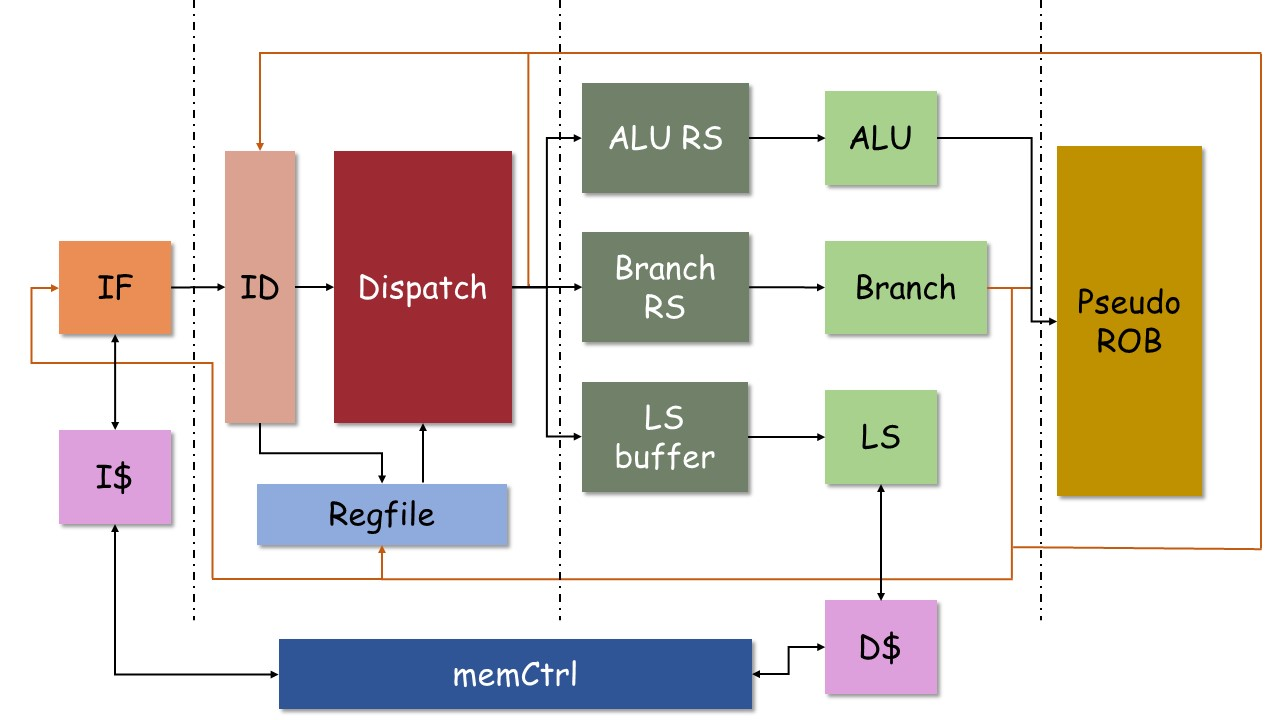
\includegraphics[width=120mm]{design.jpg}
 \end{figure}
\end{frame}

\begin{frame}{Branch Mask}
    \begin{itemize}
        \item The reason for large ALUrs and regfile is and only is logic for branch. 
        \item Faster
    \end{itemize}
    \begin{figure}
    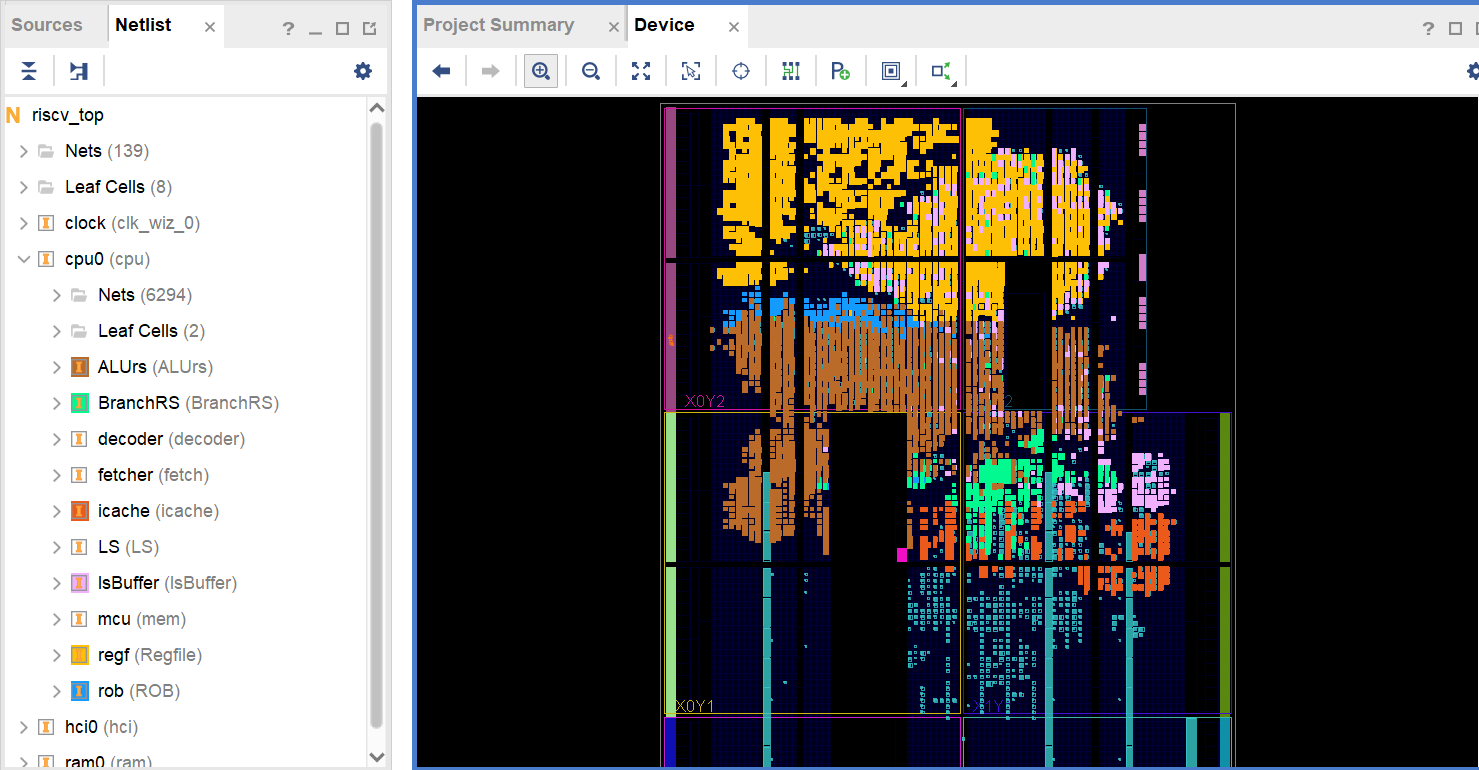
\includegraphics[width=110mm]{figure.png}
    \end{figure}
\end{frame}

\section{Pitfall}
\begin{frame}{Sometimes bigger and dumber is better?}
    Pitfall, according to CAAQA ed.6, chapter three. Pentium 4. 
    \begin{itemize}
        \item Simply adding ROB line or RS have almost no improvement; 
        \item It costs a lot to enlarge the shadow page but is obviously useless. 
        
        However, 
        
        \item Enlarging the Cache seems useless, due to the limited testbench. 
        (admitting that meeting the testbench is the most important for a design)

        Itanium 2(well, it is also a failure) and i7 vs. Pentium 4. 
    \end{itemize}
\end{frame}

\begin{frame}{And sometimes smarter is better than bigger and dumber?}
    Pitfall, according to CAAQA ed.6, chapter three. Really? 
\begin{itemize}
    \item The story of calculating head and tail in shadow register; 
    \item The story of write-back dCache. 
    
    However: 

    \item The result of branch masks; 
    \item The result of special judge when entering RS. 
\end{itemize}
    CAAQA mentions to consider the situation. 
\end{frame}

\section{Story}
\begin{frame}{My path}
    \begin{itemize}
        \item Learn and design;(6th Sep - 1st assignment)
        \item One without ROB first; 
        (after python interpreter - 23rd Nov, debug until 5th Dec)
        \item Add ROB, branch policy is stall; (23rd Nov - 9th Dec)
        \item Add branch mask, then make ROB a pseudo one to simplify. 
        Shadow regfile also;(till 15th Dec) 
        \item Add Dcache and Gshare. (1st Jan - 2nd Jan)
    \end{itemize}
\end{frame}

\begin{frame}{More stories}
    \begin{itemize}
        \item Shadow register again: only shadow tag, no shadow data: $99\%\rightarrow50\%$ LUT; 
        
        remark: considering the most complex logic, instead of the largest reg. (FF is no more than 20\%)

        \item Misprediction judgement; (more LUT but not that more, 1ns less delay)
        \item Not assign a=b, simply use b; (not elegant, but 0.7ns less delay)
        \item Only control Enable signal strictly and others loosely. 
    \end{itemize}
\end{frame}

\section{Remark}
\begin{frame}{How to judge a design?}
    \begin{itemize}
        \item testbench? 
        
        -actually not enough this time(still wrong after passing them);
        \item CPI? 
        
        -bad design can have good CPI but low frequency;

        \item Frequency and CPI? 
        
        -based on the tech of chip creation. 

        -1950s and early 1960s did not need Tomasulo. 
    \end{itemize}
    So what is this project for? A 1960 one or a 2020 one? Is Tomasulo a 2020 one? Remind Pentium 4. 
\end{frame}

\section{}
\begin{frame}
\Huge{\centerline{Thanks}}
\end{frame}

\end{document}

